%%%%%%%%%%%%%%%%%%%%%%%%%%%%%%%%%%%%%%%%%%%%%%%%%%%%%%%%%%%%%%%%%%%%%%%%%%%%%%%%
%2345678901234567890123456789012345678901234567890123456789012345678901234567890
%        1         2         3         4         5         6         7         8

%\documentclass[letterpaper, 10 pt, conference]{ieeeconf} % Comment this line out
                                                          % if you need a4paper
\documentclass[a4paper, 10pt, conference]{ieeeconf}       % Use this line for a4
                                                          % paper

\IEEEoverridecommandlockouts                              % This command is only
                                                          % needed if you want to
                                                          % use the \thanks command
\overrideIEEEmargins
% See the \addtolength command later in the file to balance the column lengths
% on the last page of the document

\usepackage{graphicx}
\graphicspath{{../data/}}

\usepackage{tikz}
\usetikzlibrary{shapes, arrows}

\usepackage{fancyvrb}
\usepackage{hyperref}

\title{\LARGE \bf
  ROS : Robotics Operating System
}

\author{
  Weipeng He
%\thanks{$^{1}$W. He is with Department of Informatics,
%        University of Hamburg, Vogt-K\"olln-Stra\ss e 30, Germany, 
%        {\tt\small 2he at informatik.uni-hamburg.de}}%
\\ Department of Informatics\\ University of Hamburg \\ {\tt\small 2he@informatik.uni-hamburg.de}
}

\begin{document}

\maketitle
\thispagestyle{empty}
\pagestyle{empty}

%%%%%%%%%%%%%%%%%%%%%%%%%%%%%%%%%%%%%%%%%%%%%%%%%%%%%%%%%%%%%%%%%%%%%%%%%%%%%%%%
\begin{abstract}
  ROS is a open-source middleware framework for developing robotics applications. It offers a large number of 
\end{abstract}


%%%%%%%%%%%%%%%%%%%%%%%%%%%%%%%%%%%%%%%%%%%%%%%%%%%%%%%%%%%%%%%%%%%%%%%%%%%%%%%%
\section{INTRODUCTION}

Software system for robots is difficult to develop because of the diversity of hardware and fast growing of its scale. Different research groups write their software for various types of robots, hardware and drivers. The software architectures they chose also differ. All these facts make the codes in robotics hard to reuse. Because of low reusability, researchers, in some cases, need to write the codes from scratch. Furthermore, the low reusability makes it hard to reproduce the experimental results from different groups.

Robot Operating System (ROS) is a project that promotes the code reuse in robotics research\cite{quigley_ros:_2009}. ROS is an open-source, meta-operating system for robots. It provides the services including hardware abstraction, low-level device control, implementation of commonly-used functionality, message-passing between processes, and package management. It also provides tools and libraries for obtaining, building, writing, and running code across multiple computers. Last but not least, ROS is supported by a open-source community (ROS.org), which is a platform for researchers to use for collaborating.

ROS was started from 2007, and now it is widely used in research and industry of robotics. Originally, it was under the name switchyard by the Stanford Artificial Intelligence Laboratory in support of the Stanford AI Robot (STAIR) project. From 2008, its development continues primarily at Willow Garage, with more than twenty institutions collaborating in a federated development model. ROS has been released several times under different distribution names. The latest stable distribution release is ``ROS Groovy Galapagos'' on December 31, 2012\cite{_documentation_2013}.

Although the latest release of ROS is targeted at Ubuntu, it also works on other linux distributions as well as Mac OS X, Android, and Windows. ROS programs can be developed in multiple programming languages, that are C++, Python, Octave and Lisp. More importantly, ROS supports more than 80 diffrent kinds of robots. The popular robots, that are PR2, Care-O-bot 3, iRobot Create, Aldebaran Nao are all included.

ROS offers plentiful modules in its repositories. It is a direct benifit for researchers to use the code from ROS rather than write the code by themselves. For example, Figure \ref{fig:tf} shows the coordinate frames in PR2, a personal service robot. The numerous moving components as well as the vision sensors have different coordinate frames. The calculation of transformation between frames is complex but essential for controlling the robot. Although the task is complex, researchers can build their programs directly based on the tf package from ROS, which reduces their workload.

\begin{figure}[htpb]
  \centering
  \includegraphics[width=.48\textwidth]{tf_pr2}
  \caption{Coordinate frames in PR2. The tf package from ROS provides algorithms for calculating transformation between multiple frames (from \cite{_documentation_2013}).}
  \label{fig:tf}
\end{figure}

Previously, there were other robotics software frameworks used in academia and industry\cite{kramer_development_2007}. Each framework was designed for some special robots or for few special tasks. Among those frameworks, Player/Stage\cite{collett_player_2005} is most similar to ROS. It is also an open-source project, and offers modules for freqently-used robotics applications. Player/Stage fits for simple, non-articulated mobile platforms. ROS, however, is better at dealing with complex mobile manipulation platforms. Furthermore, ROS offers more implementations of robotics-related algorithms.

In later sections of this paper, we will introduce the design goals, software structure and the community management of ROS. 

\section{DESIGN GOALS}

ROS is designed to solve the challenges encountered when developing large-scale service robots\cite{quigley_ros:_2009}. Its design goals are listed as follow:
\begin{itemize}
  \item Peer-to-peer
  \item Tools-based
  \item Multi-lingual
  \item Thin
  \item Free and Open-Source
\end{itemize}

\subsection{Peer-to-Peer}

ROS is designed to work on multiple hosts and processes that are connected in a peer-to-peer topology. This design avoids the using of central server, which might cause problems when working on computers in a heterogenous network. A typical working environment of ROS is shown in Figure \ref{fig:network}.

\begin{figure}[htpb]
  \centering
  \includegraphics[width=0.48\textwidth]{network}
  \caption{A typical ROS network configuration (from \cite{quigley_ros:_2009}).}
  \label{fig:network}
\end{figure}

\subsection{Tools-based} 

ROS exploits a large number of light tools to manage the building, debugging and monitoring of the programs. ROS systems, which are complex combinations of different components, need these tools to make ROS easy to use for developers.

\subsection{Multi-lingual}

ROS currently supports four programming languages: C++, Python, Octave and Lisp. This adaptation of mulitple languages meets the different language preference of programmers. Using the preferred language will large shorten the programming time and make debuggin easy.

\subsection{Thin}

While excluding standalone libraries, the core functionality of ROS is considerably thin. Most standalone libraries including those fore drivers are independent to ROS. The design of the framework shows capability to adapt code from a number of other open-source projects. For example, ROS re-uses code for the drivers, navigation system, and simulators from the Player project, vision algorithms from OpenCV, and so on. Ease for unit testing is also an benifit for thin design.

\subsection{Free and Open-Source}

ROS is a fully open platform and distributed under BSD license. It is escpecially important for researchers in robotics to colaborate, as the hardwares and functions are highly complex. ROS offers the platform for researchers to share their implementations of robotics applications.

\section{SOFTWARE STRUCTURE}

\subsection{ROS Computation Graph}
The ROS runtime ``graph'' is a peer-to-peer network of processes using the ROS communication infrastructure. Figure \ref{fig:framework}is a computatoin graph of a simple grasping application.

As shown in the graph, the ellipses are the nodes, which performs the calculation. The node are identified by their names, which also indicates their functinality. Node \texttt{/gscam} is the program for getting images from a webcam. Node \texttt{/object\_detect} is for detecting objects from images. Node \texttt{/image\_view} is for viewing an images stream. Node \texttt{/grasp} is the program for the robot to grasp the object. Node \texttt{/rosout} displays the output info of each node.

The nodes are connected via peer-to-peer links, either follow TCP or UDP protocol. The form of the connection can be two types, topic or service. In this example, there are three topics, namely \texttt{/image}, \texttt{/pos} and \texttt{/rosout}. One node can send out topic to more than one node (example is topic \texttt{/image}), and one node can also receive topics from multiple nodes (example is node \texttt{/rosout}). 

The workflow of the sample system can be described as : The webcam, controlled by node \texttt{/gscam}, gets the images and sends to node \texttt{/object\_detect} and node \texttt{/image\_view} via topic \texttt{/image}. The topic \texttt{/image} contains the data of the images taking from the webcam. The images are shown to users using node \texttt{/image\_view}. At the same time, the images are also processed by node \texttt{/object\_detect}. The position of the object is found and send to topic \texttt{/pos}. The position information is later used by node \texttt{/grasp}, and the grasping is performed. During the process, all output info are displayed in the console via topic \texttt{/rosout}.

The detailed communicating machanisms are discussed as follow.

\begin{figure}[htpb]
  \centering
  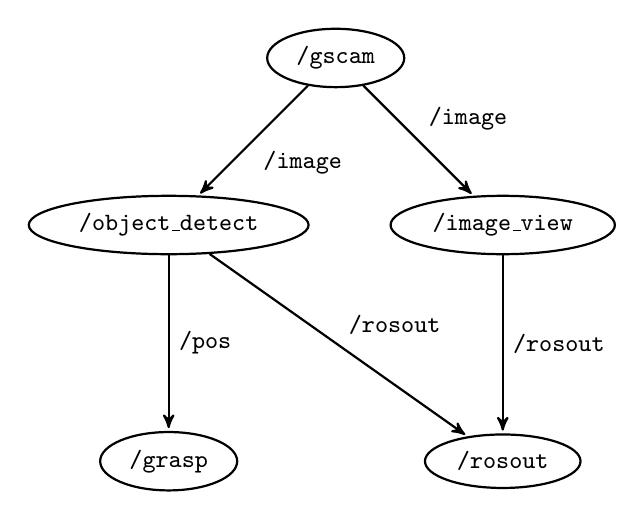
\begin{tikzpicture}[->,>=stealth',shorten >=1pt,auto,node distance=3cm,
                     thick,main node/.style={ellipse,draw,font=\ttfamily\small}]

  \node[main node] (1) {/gscam};
  \node[main node] (2) [below left of=1] {/object\_detect};
  \node[main node] (3) [below right of=1] {/image\_view};
  \node[main node] (4) [below of=3] {/rosout};
  \node[main node] (5) [below of=2] {/grasp};

  \path[every node/.style={font=\ttfamily\small}]
   (1) edge node {/image} (2)
       edge node {/image} (3)
   (2) edge node {/rosout} (4)
       edge node {/pos} (5)
   (3) edge node {/rosout} (4);
  \end{tikzpicture}
  \caption{Peer-to-peer computation graph under ROS framework. The sample system is designed for grasping objects.}
  \label{fig:framework}
\end{figure}



\subsection{Node and Master}

Nodes are independent processes that perform computation. Nodes are designed to be modular at a fine-grained scale. Robot control system will usually comprise many nodes.

The use of nodes in ROS provides several benefits to the overall system. There is additional fault tolerance as crashes are isolated to individual nodes. Code complexity is reduced in comparison to monolithic systems. Implementation details are also well hidden as the nodes expose a minimal API to the rest of the graph and alternate implementations, even in other programming languages, can easily be substituted. 

Nodes, which are identified by thier names, get to know each other via roscore, aka master. The master works as a name server. All running nodes register their name, address, port and other information at the master. Therefore, the information of other nodes can be acquired by inquisition to the master. Once these nodes have located each other, they communicate with each other peer-to-peer. The structure is shown in Figure \ref{fig:master}.

\begin{figure}[htpb]
  \centering
  \includegraphics[width=.4\textwidth]{nodes}
  \caption{roscore (master) provides the naming and registry service in ROS.}
  \label{fig:master}
\end{figure}

\subsection{Message}

Nodes communicate with each other by passing messages. Nodes receive and pass different types of data, such as a 2-D position, an image or a string message. A message work as a protocol which speicify how the structure of the tranmitted data are.

A message is simply a data structure, comprising typed fields. Standard primitive types (integer, floating, boolean, string) are supported, as are arrays of primitive types. Messages can include arbitrarily nested structures and arrays, like C structs.

Data structures of messages are specified in \texttt{.msg} files. Figure \ref{fig:message} shows the \texttt{.msg} file of built-in message \texttt{sensor\_msg/Image}. The message specifies data of a image.

\begin{figure}[htpb]
  \centering
\begin{Verbatim}[frame=single]
Header header 
  uint32 seq 
  time stamp 
  string frame_id 
uint32 height 
uint32 width 
string encoding 
uint8 is_bigendian 
uint32 step 
uint8[] data
\end{Verbatim}
  \caption{Message specification of a image. The message name is \texttt{sensor\_msg/Image}.}
  \label{fig:message}
\end{figure}

\subsection{Topic}

Topic is a mechanism for sending messages from nodes to nodes. It follows a publisher-subscriber design pattern. Publisher is the node which send messages to the topic. Subscribers are the nodes which get called whenever a message is published. The connection is unidirectional.

A topic can be viewed as a bus that connects nodes, which send out or receives the same type of data. Multiple nodes can connect to one topic simutaneously as publishers. Similarly, any node, which is interested in getting the data (messages), can connect as subscriber. Figure 
\ref{fig:topic} illustrates the concept of connecting nodes using topic.

\begin{figure}[htpb]
  \centering
  \includegraphics[width=0.48\textwidth]{topic}
  \caption{A topic can have multiple publishers and subscribers.}
  \label{fig:topic}
\end{figure}

Each topic has a strict type defined by a message type, namely a \texttt{.msg} file. As like nodes, topics are identified by their names and registered at the master. Upon a node subscribing a topic, the MD5 codes of the \texttt{.msg} files are checked for consistency of the message types.

Example of topics are discussed prviously (see Figure \ref{fig:framework}). The topic \texttt{/image} contains stream of \texttt{sensor\_msg/Image} messages, which are data of captured images from the webcam. It has one publisher, \texttt{/gscam}, and two subscribers, \texttt{/object\_detect} and \texttt{/image\_view}. The topic \texttt{/rosout}, on the other hand, is an example shows that one topic can have multiple publishers.

\subsection{Service}

Service is another type of communication between nodes. Its mechanism is a node sending a request to another node and receiving a response in return. It follows a request-response design pattern. A service is called with a request message, and a response message is returned. Figure \ref{fig:service} shows the relations bewteen nodes communicating with service.

\begin{figure}[htpb]
  \centering
  \includegraphics[width=0.48\textwidth]{service}
  \caption{A service call consists of a request and a respond.}
  \label{fig:service}
\end{figure}

A \texttt{.srv} file defines a service type. It comprises simple two parts : a request message type and a response message type. Figure \ref{fig:srvfile} is an example of a \texttt{.srv} file definition of a service, which adds two input integers (a and b) and returns the sum. The lines above the ``\texttt{---}'' are the definition of the request message type. And below it, is the definition of the response message type. Both parts can be empty (corresponding to void input and void return).

\begin{figure}[htpb]
  \centering
\begin{Verbatim}[frame=single]
int64 a
int64 b
---
int64 sum
\end{Verbatim}
  \caption{A sample \texttt{.srv} file defines the service of adding two integers.}
  \label{fig:srvfile}
\end{figure}

  Services differ from topics in several aspects. The main difference is that connections of services are bi-directional, while those of topics are uni-directional. Services can be requested with input parameters. On the contrary, topics do not have the input part. Publishers of topics send out messages without knowing the subscribers. Additionally, topics allow multiple nodes communicating at the same time, while services are between two nodes. And, the servers in services only process upon requests. However, the publishers in topics work throughout the runtime (processing may be invoked by clock). Users have the chance to decide which method to use, in order to fit their situation.

\subsection{File System Hierarchy}

ROS system on disk consists of a hierarchical filesystem. The filesystem concepts (from large to small) are stacks, packages, nodes, messages and services.

A stack is a full application suite, comprised of a collection of packages. For example, \texttt{geometry} is a stack holding libraries for geometric and mathematic computing. This stacks contains packages \texttt{tf}, \texttt{tf\_conversions}, \texttt{kdl\_conversions}, \texttt{angles} and \texttt{eigen\_conversions}.

A package is a software that solves a specific task. A package may contains several nodes. For example, the package \texttt{tf} in stack \texttt{geometry} is the package that let users keep track of multiple coordinate frames over time (in Figure \ref{fig:tf}).
  
A node, as introduced previously, is an executable in the filesystem. At runtime, a node is an independent process in the whole compuatation graph.

\section{COMMUNITY MANAGEMENT}

\subsection{Software Distribution}

   ROS code is maintained in a decentralized federation of repositories.
  
     The core repository : ros-pkg;
     94 repositories in other institutions;
     14 personal repositories.
  
   Easy to contribute.
  
     Host their code (and documents) in their own repository.
     SourceForge.net, Google Code and GitHub.
     Register at ros.org.
  
   Easy to search software.
  
     Search across the federation of repositories is possible.
     ros.org keeps tracks of updates of all repositories and generates index.
     Documentation and tutorials are also updated automatically.


   ROS Answers.

\begin{center}
  \includegraphics[width=\textwidth]{ros_answers}
\end{center}


\section{CONCLUSION}

   ROS defines a standard for the communicate mechanisms and protocols between robot components.
   ROS provides libraries for various functions.
   ROS contains utility tools to help development.
   ROS promotes code sharing and reuse.


\bibliography{ref}
\bibliographystyle{plain}  

\end{document}
